\chapter{System Overview and Objectives}
To demonstrate the efficacy of a source synchronous system we use a single
receiver that receives data from two different channels.  The two channels
would transmit a pseudorandom binary sequence (PRBS), from a single source. At
set intervals the source alternates the channel over which it transmits.  Hence
the overall effect is that the channels would optically transmit bursts of data
at non-overlapping intervals. If the receiver is successfully able to receive
the full sequence, then the source synchronous system would be working
correctly.  An overview of the system is shown in
Figure~\ref{fig:overview}. 

\begin{figure}[h]
    \centering
    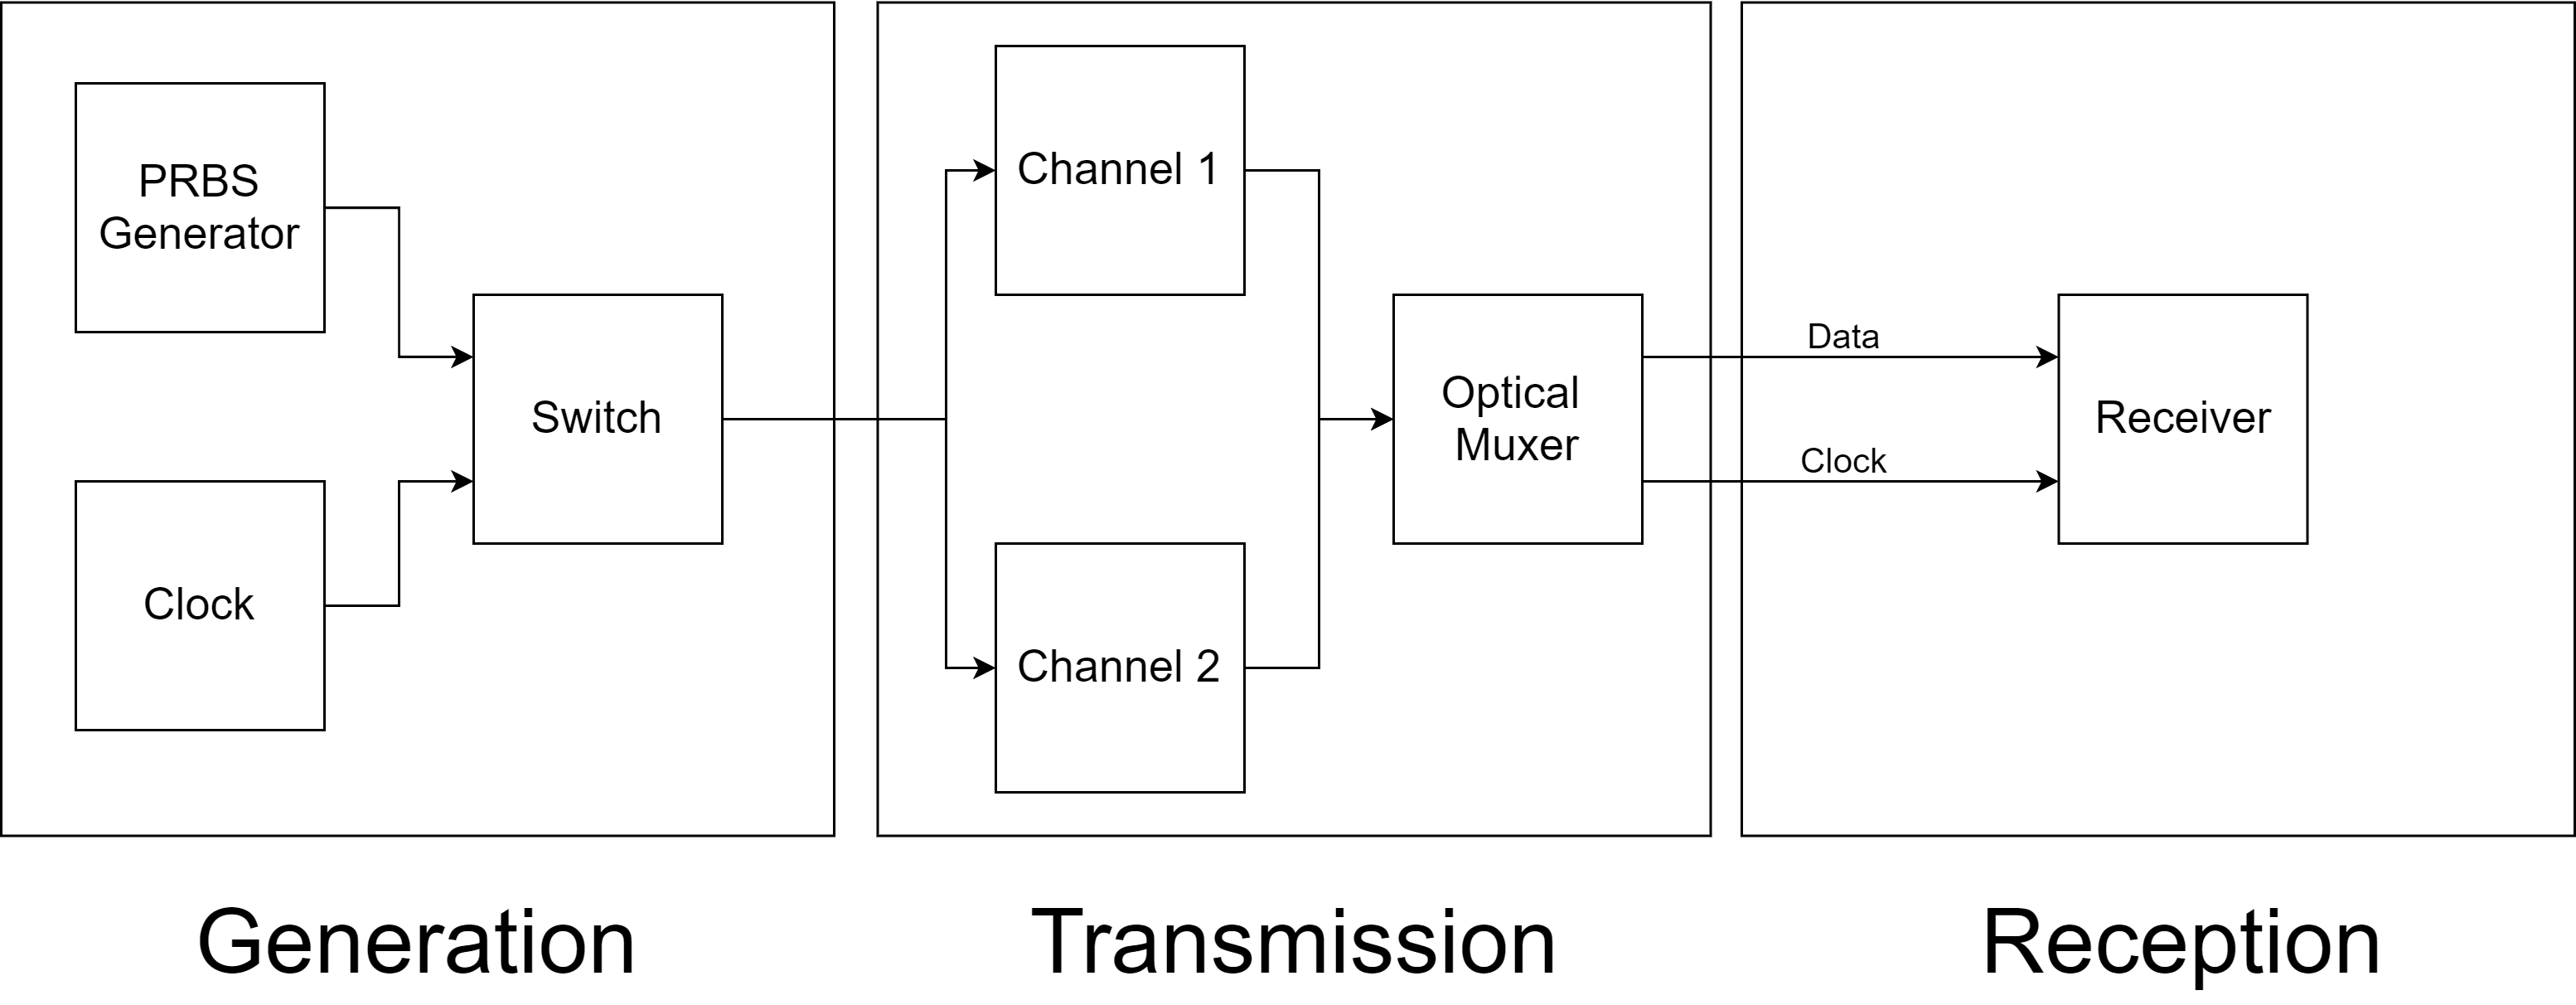
\includegraphics[width=1\linewidth]{img/overview.png}
    \caption{Overview of System}%
    \label{fig:overview}
\end{figure}

The overall objective is to demonstrate successful burst source synchronous
communication.  If successful, we would then be able to compare the throughput
of the system with a similar system that utilised a CDR circuit.

To accomplish this the following components are needed:
\begin{itemize}
    \item A burst mode PRBS generator
    \item An optical switch 
    \item Source synchronous PRBS checker 
\end{itemize}

